\documentclass[]{article}
\newcommand{\FileDepth}{../../..}
\usepackage[letterpaper, landscape, margin=0.5cm]{geometry}
\usepackage[T1]{fontenc}
\usepackage{textcomp}%Not strictly necessary, but gives \textmu command for "micro."
\usepackage{fancyhdr}
\usepackage{amsmath}
\usepackage{amssymb}
\usepackage{graphicx}
\usepackage{xcolor}
\usepackage{tikz}
\usetikzlibrary{calc}
\usepackage[shortlabels]{enumitem}
\usepackage{multicol}
\usepackage{vwcol}
\usepackage{hyperref}
\usepackage{wrapfig}
%opening
\newcommand{\SecType}{L}
\newcommand{\Week}{9}
\title{PH 211 Lecture \Week}
\author{Benjamin Bauml}
\date{Summer 2024}

\newcommand{\Purpose}{4}
\newcommand{\DefOnly}{0}

\input{\FileDepth/Formats/Assignment20240614.tex}
\usepackage[absolute]{textpos}
% This package relies on Assignment Format 2024-06-14 or later to work. It is recommended that the Purpose and DefOnly commands be given as such:
%\newcommand{\Purpose}{4}
%\newcommand{\DefOnly}{0}
% Activities need to be entered outside of the TeacherMargin and PresentSpace environments, otherwise they will be defined only locally. They can even go in the preamble.
\newenvironment{TeacherMargin}{\begin{textblock*}{10.8cm}(0.5cm,0.5cm)
\small}{\end{textblock*}
\hspace{0.1cm}}
\newenvironment{PresentSpace}{\begin{textblock*}{0.3cm}(26.85cm,9.35cm)
--
\end{textblock*}
\begin{textblock*}{15.6cm}(11.8cm,0.5cm)
\begin{Repurpose}{1}
\Large}{\end{Repurpose}
\end{textblock*}
\hspace{0.1cm}}

\newcommand{\FBDaxes}[4][2]{
	\begin{scope}[shift={(#2)},rotate=#3]
		% x-axis
		\draw[thick,->] (-#1,0) -- (#1,0);
		\node[anchor=west] at (#1,0) {$x$};
		% y-axis
		\draw[thick,->] (0,-#1) -- (0,#1);
		\node[anchor=south] at (0,#1) {$y$};
		\coordinate (#4) at (0,0);
	\end{scope}
}
\newcommand{\FBDvectorMA}[4]{
	\begin{scope}[shift={(#1)}]
		\coordinate (#4tip) at ({#2*cos(#3)},{#2*sin(#3)});
		\draw[ultra thick,blue,->] (#1) -- (#4tip);
	\end{scope}
}
\newcommand{\FBDvectorXY}[3]{
	\begin{scope}[shift={(#1)}]
		\coordinate (#3tip) at (#2);
		\draw[ultra thick,blue,->] (0,0) -- (#3tip);
	\end{scope}
}
\newcommand{\FBDdot}[1]{
	\filldraw[black] (#1) circle (3pt);
}
\newcommand{\FBDbox}[5][1]{
	\begin{scope}[shift={(#2)},rotate=#3]
		\filldraw[color=black,fill=white,thick] ({-#1/2},{#1/2}) -- ({-#1/2},{-#1/2}) -- ({#1/2},{-#1/2}) -- ({#1/2},{#1/2}) -- cycle;
		% Left side coordinates
		\coordinate (#4ltq) at ({-#1/2},{#1/4});
		\coordinate (#4lcent) at ({-#1/2},0);
		\coordinate (#4lbq) at ({-#1/2},{-#1/4});
		% right side coordinates
		\coordinate (#4rtq) at ({#1/2},{#1/4});
		\coordinate (#4rcent) at ({#1/2},0);
		\coordinate (#4rbq) at ({#1/2},{-#1/4});
		% top coordinates
		\coordinate (#4tlq) at ({-#1/4},{#1/2});
		\coordinate (#4tcent) at (0,{#1/2});
		\coordinate (#4trq) at ({#1/4},{#1/2});
		% bottom coordinates
		\coordinate (#4blq) at ({-#1/4},{-#1/2});
		\coordinate (#4bcent) at (0,{-#1/2});
		\coordinate (#4brq) at ({#1/4},{-#1/2});
		% corners
		\coordinate (#4tl) at ({-#1/2},{#1/2});
		\coordinate (#4tr) at ({#1/2},{#1/2});
		\coordinate (#4bl) at ({-#1/2},{-#1/2});
		\coordinate (#4br) at ({#1/2},{-#1/2});
		\node at (0,0) {#5};
	\end{scope}
}
%\newcommand{\MVec}[3][0]{%Creates a momentum vector of length #3 centered at #2 and rotated #1 degrees counterclockwise.
	\begin{scope}[rotate=#1,shift={(#2)}]
		\draw[->,thick] ({-#3/2},0) -- ({#3/2},0);
	\end{scope}
}
\newcommand{\MDot}[1]{%Creates a dot at #1 to represent a zero vector.
	\filldraw (#1) circle (1pt);
}
\newcommand{\MVDRows}[2][4.5]{%Creates the rows (initial, delta, final) of a momentum vector diagram. The optional argument determines the width of the table, and defaults to a good length for three columns (two objects and the total system). The non-optional argument gives a coordinate name (not displayed) to the diagram.
	\begin{scope}
		%\draw[thick] (0,5.5) -- (0,0);
		\draw[thick] (-1,4.5) -- (#1,4.5);
		\node at (-0.5,3.75) {$\vec{p}_{i}$};
		\draw[thick] (-1,3) -- (#1,3);
		\node at (-0.5,2.25) {$\Delta\vec{p}$};
		\draw[thick] (-1,1.5) -- (#1,1.5);
		\node at (-0.5,0.75) {$\vec{p}_{f}$};
		\coordinate (#2) at (0,5);
	\end{scope}
}
\newcommand{\MVDCol}[4][0.75]{%Creates a column for an object in a momentum vector diagram. The first (non-optional) argument is the coordinate name (not displayed) of the column, while the second is the displayed column header. The first argument also names the three entries down the column. The third argument anchors the column, so it should either be the coordinate name of the MVD (for the first column) or the coordinate name of the previous column. The optional argument indicates how far the center of the column should be from the previous column's edge, and defaults to 0.75.
	\begin{scope}[shift={(#4)}]
		\node at (#1,0) {#3};
		%\draw[thick] ({#1*2},0.5) -- ({#1*2},-5);
		\draw[thick] (0,0.5) -- (0,-5);
		\coordinate (#2init) at (#1,-1.25);
		\coordinate (#2delt) at (#1,-2.75);
		\coordinate (#2fin) at (#1,-4.25);
		\coordinate (#2) at ({#1*2},0);
	\end{scope}
}

%\input{\FileDepth/Activities/Activity_One/Activity_One.tex}
%\input{\FileDepth/Activities/Activity_Two/Activity_Two.tex}

\begin{document}
\begin{TeacherMargin}

\end{TeacherMargin}
\begin{PresentSpace}
\begin{center}
	\huge Lecture 9: Static Special Cases
\end{center}
\vspace{0.5cm}
\underline{In-Class Quizzes on Monday}
\begin{itemize}
	\item Two Quizzes: Motion and Forces
	\begin{itemize}
		\large
		\item Formatted just like the practice quizzes in the Week 3 module.
		\item Not just calculations; could be assumptions, sensemaking, explanations, etc.
	\end{itemize}
	\item One sheet (front and back) of notes allowed.
	\item Scientific calculators only (no graphing calculators).
	\begin{itemize}
		\large
		\item There will be some some numerical calculation, but it is not a major emphasis.
	\end{itemize}
	\item For simplicity, $g\approx 10$ m/s$^{2}$.
\end{itemize}
\vspace{0.5cm}
\underline{Other Announcements}
\begin{itemize}
	\item Working on another back-up lecture location.
	\begin{itemize}
		\large
		\item Main classroom will still be WNGR 212.
		\begin{itemize}
			\item Hopefully here for quizzes, but maybe BEXL 103 if it is still too warm (won't know until Monday).
		\end{itemize}
		\item May have to change ``official'' classroom to reserve a back-up room for the term.
	\end{itemize}
	\item Don't forget the Address Assessment portion of your lab reports.
	\begin{itemize}
		\item This will make your lab feedback more effective by helping your TA see how you are trying to improve.
	\end{itemize}
	\item Let us know how if you have issues with the feedback you receive on assignments.
	\begin{itemize}
		\large
		\item Is it clear? Is it enough? How is the tone? Other thoughts?
	\end{itemize}
\end{itemize}
\end{PresentSpace}
\newpage
\begin{TeacherMargin}
\noindent\textbf{(A)}
\begin{center}
	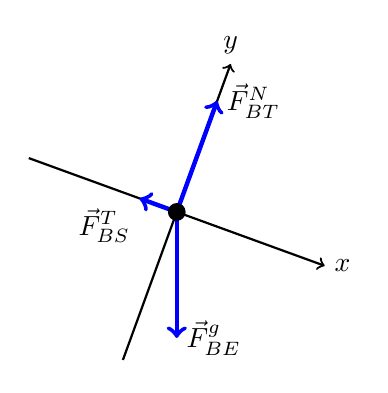
\begin{tikzpicture}
		\FBDaxes{0,0}{-20}{axes}
		\FBDvectorMA{axes}{1.5}{70}{FN}
		\node[anchor=west] at (FNtip) {$\vec{F}^{N}_{BT}$};
		\FBDvectorMA{axes}{1.6}{-90}{FG}
		\node[anchor=west] at (FGtip) {$\vec{F}^{g}_{BE}$};
		\FBDvectorMA{axes}{0.5}{160}{FT}
		\node[anchor=north east] at (FTtip) {$\vec{F}^{T}_{BS}$};
		\FBDdot{axes}
	\end{tikzpicture}
\end{center}
\noindent\textbf{(B)} 
In this problem, it makes sense to tilt the axes. By aligning the normal force with the $y$-axis and the tension force with the (negative) $x$-axis, we now don't have to break them into components: $F^{N}_{BT,y}=F^{N}_{BT}$ and $F^{T}_{BS,x}=-F^{T}_{BS}$. That leaves just one vector to break up: the force of gravity.
\begin{center}
	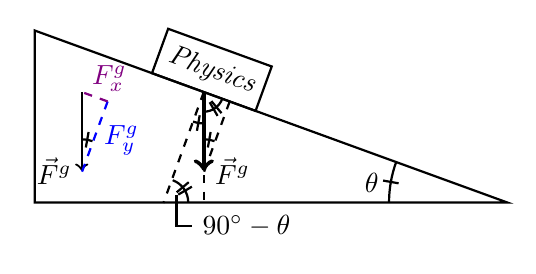
\begin{tikzpicture}
		\draw[thick] (-6,0) -- (0,0) -- (-6,{6*tan(20)}) -- cycle;
		\draw[thick] (-1.5,0) node[anchor=south east] {$\theta$} arc (180:160:1.5);
		\draw[thick,rotate=-10] (-1.6,0) -- (-1.4,0);
		\draw[thick,rotate=-20] (-4.8,0) node[anchor=south west,rotate=-20] {\textit{Physics}} rectangle (-3.4,0.6);
		\draw[ultra thick,->] ({-4.1*cos(20)},{4.1*sin(20)}) -- ({-4.1*cos(20)},{4.1*sin(20)-1}) node[anchor=west] {$\vec{F}^{g}$};
		\draw[thick,shift={({-4.1*cos(20)},{4.1*sin(20)})}] (0,-0.25) arc (270:340:0.25);
		\draw[thick,shift={({-4.1*cos(20)},{4.1*sin(20)})},rotate=30] (0,-0.15) -- (0,-0.35);
		\draw[thick,shift={({-4.1*cos(20)},{4.1*sin(20)})},rotate=40] (0,-0.15) -- (0,-0.35);
		\draw[thick,dashed] ({-4.1*cos(20)},{4.1*sin(20)}) -- ({-4.1*cos(20)},0);
		\draw[thick] ({-4.1*cos(20)},{4.1*sin(20)-0.6}) arc (90:70:0.4);
		\draw[thick,shift={({-4.1*cos(20)},{4.1*sin(20)-1})},rotate=-10] (0,0.3) -- (0,0.5);
		\draw[thick] ({-4.1*cos(20)},{4.1*sin(20)-0.4}) arc (270:250:0.4);
		\draw[thick,shift={({-4.1*cos(20)},{4.1*sin(20)})},rotate=-10] (0,-0.3) -- (0,-0.5);
		\draw[thick,dashed,rotate=-20] (-3.75,0) -- (-3.75,-1);
		\draw[thick,dashed,rotate=-20] (-4.1,0) -- (-4.1,-1.5);
		\draw[thick] (-4.05,0) arc (0:70:0.3);
		\draw[thick] (-4.2,0.1) -- (-4.2,-0.3) -- (-4,-0.3) node[anchor=west] {$90^{\circ}-\theta$};
		\draw[thick,shift={(-4.35,0)},rotate=40] (0.2,0) -- (0.4,0);
		\draw[thick,shift={(-4.35,0)},rotate=30] (0.2,0) -- (0.4,0);
		\begin{scope}[shift={(-1.55,0)}]
			\draw[thick,->] ({-4.1*cos(20)},{4.1*sin(20)}) -- ({-4.1*cos(20)},{4.1*sin(20)-1}) node[anchor=east] {$\vec{F}^{g}$};
			\draw[thick] ({-4.1*cos(20)},{4.1*sin(20)-0.6}) arc (90:70:0.4);
			\draw[thick,shift={({-4.1*cos(20)},{4.1*sin(20)-1})},rotate=-10] (0,0.3) -- (0,0.5);
			\draw[thick,dashed,rotate=-20,blue] (-3.75,0) node[anchor=north,shift={(5pt,-5pt)}] {$F^{g}_{y}$} -- (-3.75,-1);
			\draw[thick,dashed,rotate=-20,violet] (-3.75,0) -- (-4.1,0) node[anchor=west,shift={(0,5pt)}] {$F^{g}_{x}$};
		\end{scope}
	\end{tikzpicture}
\end{center}
There are a number of right triangles in the figure above that can help us determine that
\begin{align*}
	F^{g}_{BE,x} & = F^{g}_{BE}\sin\theta, & F^{g}_{BE,y} & = -F^{g}_{BE}\cos\theta.
\end{align*}
We can also determine this with special-case analysis. We should get $\vec{F}^{g} = -F^{g}\hat{y}$ when $\theta=0^{\circ}$ (our standard coordinate system) and $\vec{F}^{g} = F^{g}\hat{x}$ when $\theta=90^{\circ}$ (tilted such that $\hat{x}$ points down). We can guess where the signs and trigonometric functions go and check these special cases, which will eliminate equations for $\vec{F}^{g}$ that don't behave correctly.

\noindent\textbf{(C)} 
The net force on the book should be zero, as the book is not accelerating. The string is keeping the book from moving along the surface, and the book doesn't fall through or leap off of the table.

\noindent\textbf{(D)} 
We know that $\vec{F}^{net} = \vec{0}$. In the $x$-direction, this tells us:
\begin{align*}
	0 = F^{net}_{x} & = F^{g}_{BE,x} + F^{T}_{BS,x} \\
	& = F^{g}_{BE}\sin\theta - F^{T}_{BS} \\
	& \implies F^{T}_{BS} = F^{g}_{BE}\sin\theta
\end{align*}
In the $y$-direction, this tells us:
\begin{align*}
	0 = F^{net}_{y} & = F^{g}_{BE,y} + F^{N}_{BT,y} \\
	& = -F^{g}_{BE}\cos\theta + F^{N}_{BT} \\
	& \implies F^{N}_{BT} = F^{g}_{BE}\cos\theta
\end{align*}
\end{TeacherMargin}
\begin{PresentSpace}
\vspace{-10pt}
\section*{L9-1: Textbook on a Tilted Table}
\vspace{-10pt}
A physics textbook is on a tilted, frictionless table, supported by a string.
\begin{enumerate}[(A)]
	\item Sketch a free-body diagram for the system.
	\item What coordinate system do you think will \\
	make analyzing this situation easiest?
	\item Should the net force on the book be \textit{zero} or \\
	\textit{not zero}?
	\item Write an expression for the magnitude of each force acting on the system in terms of the gravitational force $F^{g}$.
\end{enumerate}
\end{PresentSpace}
\begin{textblock*}{5cm}(22cm,3cm)
\centering
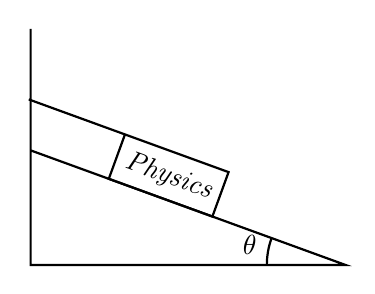
\begin{tikzpicture}
	\draw[thick] (-4,3) -- (-4,0) -- (0,0) -- (-4,{4*tan(20)});
	\draw[thick] (-1,0) node[anchor=south east] {$\theta$} arc (180:160:1);
	\draw[thick,rotate=-20] (-3.2,0) node[anchor=south west,rotate=-20] {\textit{Physics}} rectangle (-1.8,0.6);
	\draw[thick,rotate=-20] (-3.2,0.6) -- (-4.5,0.6);
\end{tikzpicture}
\end{textblock*}
\newpage
\begin{TeacherMargin}

\end{TeacherMargin}
\begin{PresentSpace}
\vspace{-10pt}
\section*{Special-Case Analysis}
\vspace{-10pt}
After you solve for a quantity:
\begin{itemize}
	\item Choose a case that is special, not arbitrary.
	%\begin{itemize}
	%	\item \textit{Example: What if the ramp were vertical/horizontal?}
	%\end{itemize}
	\item Figure out what your quantity \textbf{should} be in the case you chose.
	%\begin{itemize}
	%	\item \textit{Example: What should the normal force be when the ramp is vertical/horizontal?}
	%\end{itemize}
	\item Identify the value of one or more other quantities that corresponds to your \textbf{case}.
	%\begin{itemize}
	%	\item \textit{Example: What is the value of $\theta$ if the ramp is vertical/horizontal?}
	%\end{itemize}
	\item Evaluate your answer in the special case.
	\item Check whether or not your symbolic answer for the case matches what you expected the answer should be.
\end{itemize}
\end{PresentSpace}
\newpage
\begin{TeacherMargin}
\noindent\textbf{Increased Verticality (Covariational Sensemaking)} \\
As the table tilts more, the string has to support the book more and more to keep it from sliding, and the surface of the table correspondingly needs to support the book less and less. Thus, the magnitude of the normal force will decrease, and the magnitude of the tension force will increase.

Note that $\cos\theta$ decreases and $\sin\theta$ increases as $\theta$ increases, so our symbolic answers agree with our physical prediction.

\noindent\textbf{Horizontal Case (Special-Case Analysis)} \\
When the table is flat ($\theta=0^{\circ}$), the string does not need to pull on the book to keep it from sliding. The tension will be 0 N, and the normal force will be equal in magnitude to the force of gravity. Our symbolic answers agree with this expectation:
\begin{align*}
	F^{T}_{BS} & = F^{g}_{BE}\sin(0^{\circ}) = 0\text{ N} \\
	F^{N}_{BT} & = F^{g}_{BE}\cos(0^{\circ}) = F^{g}_{BE}
\end{align*}
\textbf{Vertical Case (Special-Case Analysis)} \\
When the table is vertical ($\theta=90^{\circ}$), the string is supporting the entire weight of the book, and the surface of the table does not support the boook at all (the book just hangs beside it from the string). The tension is equal in magnitude to the force of gravity, and the normal force will be 0 N. Our symbolic answers agree with this expectation:
\begin{align*}
	F^{T}_{BS} & = F^{g}_{BE}\sin(90^{\circ}) = F^{g}_{BE} \\
	F^{N}_{BT} & = F^{g}_{BE}\cos(90^{\circ}) = 0\text{ N}
\end{align*}
\end{TeacherMargin}
\begin{PresentSpace}
\vspace{-10pt}
\section*{L9-2: Tilted Table Sensemaking}
\vspace{-10pt}
A physics textbook is on a tilted, frictionless table, supported by a string.
\begin{itemize}
	\item Suppose the table is slanted so that it becomes \textit{steeper}. What happens to the magnitudes of the normal force \\
	and the tension force?% Do they \textit{increase}, \\
	%\textit{decrease}, or \textit{stay the same}?
	\begin{comment}
		\large
		\item Does the magnitude of the normal force \\
		\textit{increase}, \textit{decrease}, or \textit{stay the same}?
		\item Does the magnitude of the tension force \\ \textit{increase}, \textit{decrease}, or \textit{stay the same}?
	\end{comment}
	\item Consider the following special cases:
	\begin{itemize}
		\large
		\item What if the table were horizontal?
		\item What if the table were vertical?
	\end{itemize}
	\vspace{-8pt}
	For each of these cases, answer the following questions:
	\begin{itemize}
		\large
		\item How big \textbf{should} each force be?
		\item What angle corresponds to this \textbf{case}?
		\item Does our symbolic answer for the case match what the answer should be?
	\end{itemize}
	\begin{comment}
	\item What if the table were horizontal?
	\begin{itemize}
		\item How big \textbf{should} each force be?
		\item What angle corresponds to this \textbf{case}?
		\item Does our symbolic answer for the case match what the answer should be?
	\end{itemize}
	\item What if the table were vertical?
	\begin{itemize}
		\item How big \textbf{should} each force be?
		\item What angle corresponds to this \textbf{case}?
		\item Does our symbolic answer for the case match what the answer should be?
	\end{itemize}
	\end{comment}
\end{itemize}
\end{PresentSpace}
\begin{textblock*}{5cm}(22cm,3.25cm)
\centering
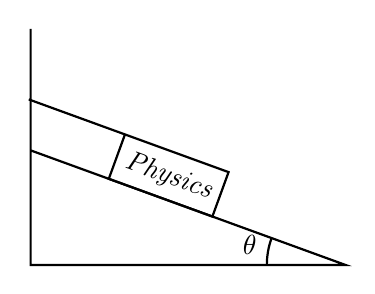
\begin{tikzpicture}
	\draw[thick] (-4,3) -- (-4,0) -- (0,0) -- (-4,{4*tan(20)});
	\draw[thick] (-1,0) node[anchor=south east] {$\theta$} arc (180:160:1);
	\draw[thick,rotate=-20] (-3.2,0) node[anchor=south west,rotate=-20] {\textit{Physics}} rectangle (-1.8,0.6);
	\draw[thick,rotate=-20] (-3.2,0.6) -- (-4.5,0.6);
\end{tikzpicture}
\end{textblock*}
\newpage
\begin{TeacherMargin}
	
\end{TeacherMargin}
\begin{PresentSpace}
\section*{Main Ideas}
\begin{itemize}
	\item Tension and normal force don't have models with which to be directly calculated, so we need to find them via Newton's 2nd law.
	\item Picking a special case for which the answer is clear by physical reasoning can be a powerful tool for checking symbolic solutions.
\end{itemize}
\end{PresentSpace}
\end{document}